\documentclass[11pt,a4paper]{article}

\usepackage[utf8]{inputenc}
\usepackage[T1]{fontenc}
\usepackage[brazil]{babel}
\usepackage{amsmath, amssymb}
\usepackage{graphicx}
\usepackage{booktabs}
\usepackage{siunitx}
\usepackage[margin=2.3cm]{geometry}
\usepackage{float}
\usepackage{caption}
\usepackage{subcaption}
\usepackage{xcolor}
\usepackage{listings}
\usepackage{tikz}
\usetikzlibrary{arrows.meta,patterns,calc,decorations.pathreplacing}
\usepackage[colorlinks=true, linkcolor=blue!55!black, citecolor=blue!55!black, urlcolor=blue!55!black]{hyperref}

\sisetup{
    output-decimal-marker = {,},
    group-digits = integer,
    group-separator = {.},
    group-minimum-digits = 4,
    per-mode = symbol
}

\captionsetup{
    font = small,
    labelfont = bf
}

\newcommand{\cab}[2]{\begin{tabular}[c]{@{}c@{}}#1\\\relax #2\end{tabular}}

% Configuracao do pacote listings com suporte UTF-8 completo para pdflatex
\definecolor{codebg}{rgb}{0.97,0.97,0.98}
\definecolor{codekw}{rgb}{0.08,0.32,0.65}
\definecolor{codecm}{rgb}{0.35,0.45,0.35}
\definecolor{codestr}{rgb}{0.68,0.18,0.18}

\lstset{
    backgroundcolor=\color{codebg},
    basicstyle=\ttfamily\scriptsize,
    aboveskip=4pt,
    belowskip=4pt,
    lineskip=-0.5pt,
    breaklines=true,
    breakatwhitespace=false,
    captionpos=b,
    commentstyle=\color{codecm}\itshape,
    keywordstyle=\color{codekw}\bfseries,
    stringstyle=\color{codestr},
    numbers=left,
    numberstyle=\tiny\color{gray},
    numbersep=6pt,
    frame=single,
    rulecolor=\color{gray!40},
    showstringspaces=false,
    tabsize=4,
    inputencoding=utf8,
    extendedchars=true,
    literate=
        {á}{{\'a}}1 {é}{{\'e}}1 {í}{{\'i}}1 {ó}{{\'o}}1 {ú}{{\'u}}1
        {Á}{{\'A}}1 {É}{{\'E}}1 {Í}{{\'I}}1 {Ó}{{\'O}}1 {Ú}{{\'U}}1
        {â}{{\^a}}1 {ê}{{\^e}}1 {ô}{{\^o}}1
        {Â}{{\^A}}1 {Ê}{{\^E}}1 {Ô}{{\^O}}1
        {ã}{{\~a}}1 {õ}{{\~o}}1 {Ã}{{\~A}}1 {Õ}{{\~O}}1
        {à}{{\`a}}1 {À}{{\`A}}1 {ç}{{\c{c}}}1 {Ç}{{\c{C}}}1
        {ü}{{\"u}}1 {Ü}{{\"U}}1
        {°}{{\textdegree}}1 {²}{{\textsuperscript{2}}}1 {³}{{\textsuperscript{3}}}1
        {–}{{-}}1 {—}{{-}}1
}

\begin{document}

% =========================================================================
% CABECALHO FORMAL EPUSP
% =========================================================================
\begin{titlepage}
    \centering
    \vspace*{0.2cm}
    
\includegraphics[width=0.28\textwidth]{figuras/logo_poli_usp.png}\\[0.6cm]
    {\large \textsc{Universidade de São Paulo}}\\[0.2cm]
    {\Large \textbf{Escola Politécnica da USP}}\\[0.2cm]
    {\normalsize Departamento de Engenharia Mecânica (PME)}\\[1.5cm]

    \rule{\linewidth}{0.8pt}\\[0.5cm]
    {\LARGE \textbf{PME 3361 -- Transferência de Calor}}\\[0.3cm]
    {\Large \textbf{Projeto I -- Avaliação de Processo de Colagem por Laser}}\\[0.3cm]
    \rule{\linewidth}{0.8pt}\\[1.2cm]

    {\Large \textbf{Grupo 15C}}\\[0.6cm]
    \begin{tabular}{ll}
        \toprule
        \textbf{Integrante} & \textbf{NUSP} \\
        \midrule
        Gabriel Barros Louro Alves & 15586270 \\
        Henrique Hideki Miashiro & 13672209 \\
        Lucas Augusto Gazotti & 15471223 \\
        Guilherme Watanabe Miyake & 14576555 \\
        \bottomrule
    \end{tabular}

    \vfill
    {\normalsize São Paulo -- SP}\\
    {\normalsize Entrega: 01 de dezembro de 2026}
\end{titlepage}

\tableofcontents
\newpage

% =========================================================================
% 1. RESUMO
% =========================================================================
\section{Resumo}
Este trabalho apresenta a modelagem matemática, a simulação numérica transiente e a análise crítica de engenharia do processo de colagem térmica de uma película plástica sobre a faixa central de uma chapa de aço via aquecimento por laser, referente ao \textbf{Grupo 15C} ($h = \SI{150}{W/(m^2.K)}$, $q'' = \SI{80000}{W/m^2}$ e $T_\infty = \SI{25}{\celsius}$). Dada a reduzida espessura da chapa ($d = \SI{1,25}{mm}$), o número de Biot transversal resulta em $\text{Bi}_y = \num{3,125e-3} \ll 0,1$, validando a hipótese de temperatura uniforme na espessura e a redução para um problema unidimensional transiente com convecção em ambas as faces e termo fonte localizado. A equação governante adimensionalizada foi resolvida pelo Método das Diferenças Finitas com aproximação centrada de 2ª ordem no espaço, tratamento da condição de simetria segundo Lomax e Pulliam e integração temporal por Euler Implícito com fatoração LU esparsa. O código foi validado contra o caso de referência do Grupo 11A ($\text{Bi} = 5,808$; $\tilde{q} = 174,240$; $T_{\max} = \SI{152,23}{\celsius}$; $T_{\text{borda}}(10\text{ s}) = \SI{93,83}{\celsius}$) e submetido a estudo de convergência espacial ($N \in \{100, 200, 400\}$) e temporal ($N_t \in \{1500, 3000, 6000\}$), exibindo desvios inferiores a \SI{1}{\percent} na malha base ($N=200, N_t=3000$). No caso base do Grupo 15C, embora a temperatura máxima no centro atinja \SI{147,80}{\celsius} sem violar o limite superior de \SI{200}{\celsius}, a borda da película ($x = \SI{22}{mm}$) alcança \SI{90}{\celsius} apenas em $t = \SI{9,78}{s}$ e termina o pulso em \SI{91,02}{\celsius}, resultando em uma janela útil de apenas \SI{0,22}{s} durante o pulso e margem térmica insuficiente (\SI{1,02}{\celsius}). Para adequar o processo, foram simuladas quatro soluções de engenharia, demonstrando que o alargamento do feixe para $w_{\text{laser}} = \SI{60}{mm}$ combinado a um pulso em dois estágios ($\SI{180}{kW/m^2}$ por $\SI{2,0}{s}$ seguido de $\SI{75}{kW/m^2}$ até $\SI{10,0}{s}$) eleva o tempo útil na janela $[\SI{90}{\celsius}, \SI{200}{\celsius}]$ para \SI{8,24}{s}, reduz o gradiente térmico na película de \SI{56,78}{\celsius} para \SI{30,61}{\celsius} e preserva uma folga de segurança de \SI{28,63}{\celsius} abaixo do limite de degradação.

% =========================================================================
% 2. DESCRICAO DO PROBLEMA
% =========================================================================
\section{Descrição do problema}
O processo industrial avaliado consiste na adesão térmica de uma película polimérica de largura $w_1 = \SI{44}{mm}$ aplicada na região central de uma fita de aço carbono de espessura $d = \SI{1,25}{mm}$, largura total $w_2 = \SI{132}{mm}$ (razão geométrica $p = w_2/w_1 = 3$) e comprimento unitário (\SI{1}{m}) ortogonal ao plano da seção transversal. Um feixe de laser incide sobre a faixa central $|x| \le w_1/2$ impondo um fluxo de calor superficial uniforme $q''$ durante um pulso de duração $\Delta t_L = \SI{10}{s}$, seguido de resfriamento livre do feixe até o instante final $t_{\text{final}} = \SI{30}{s}$. Ambas as superfícies da chapa trocam calor por convecção com o ar ambiente à temperatura $T_\infty$ e coeficiente convectivo $h$.

A Figura~\ref{fig:esquema} ilustra o domínio físico do problema e o aproveitamento da simetria geométrica e térmica em $x = 0$, restringindo o domínio de cálculo à meia chapa $0 \le x \le L = w_2/2 = \SI{66}{mm}$.

\begin{figure}[H]
    \centering
    \begin{tikzpicture}[scale=1.02, >=Stealth]
        % Eixo de simetria
        \draw[dash pattern=on 5pt off 3pt on 1pt off 3pt, thick, gray!80!black]
            (0, -1.10) -- (0, 2.40) node[above, black, font=\footnotesize] {Eixo de simetria ($x = 0$)};

        % Chapa de aco (-6.6 a +6.6 cm -> representado em [-5.4, +5.4])
        \fill[gray!25] (-5.4, 0) rectangle (5.4, 0.36);
        \draw[thick] (-5.4, 0) rectangle (5.4, 0.36);

        % Pelicula plastica central (-w1/2 a +w1/2 -> [-1.8, +1.8])
        \fill[teal!45] (-1.8, 0.36) rectangle (1.8, 0.52);
        \draw[thick, teal!60!black] (-1.8, 0.36) rectangle (1.8, 0.52);
        \node[teal!50!black, font=\footnotesize, anchor=center] (pel) at (-3.35, 1.36) {Película ($w_1 = \SI{44}{mm}$)};
        \draw[->, thin, teal!60!black] (pel.south east) -- (-1.65, 0.53);

        % Setas e rotulo do laser q''
        \foreach \x in {-1.5, -1.0, -0.5, 0.0, 0.5, 1.0, 1.5} {
            \draw[->, red!80!black, thick] (\x, 1.52) -- (\x, 0.56);
        }
        \node[red!80!black, font=\small\bfseries, fill=white, inner sep=2pt] at (0, 1.88) {$q''\;(\Delta t_L = \SI{10}{s})$};

        % Conveccao na face superior
        \draw[->, blue!70!black] (-4.6, 0.88) -- (-4.6, 0.42);
        \draw[->, blue!70!black] (3.3, 1.02) -- (3.3, 0.42);
        \draw[->, blue!70!black] (4.3, 1.02) -- (4.3, 0.42);
        \node[blue!70!black, font=\footnotesize] at (3.8, 1.25) {Convecção: $h, T_\infty$};

        % Conveccao na face inferior (fora da faixa central da cota w1)
        \foreach \x in {-4.4, -2.7, 2.7, 4.4} {
            \draw[->, blue!70!black] (\x, -0.78) -- (\x, -0.06);
        }
        \node[blue!70!black, font=\footnotesize] at (3.55, -1.00) {Convecção: $h, T_\infty$};

        % Extremidades a T_inf (acima das pontas, sem conflito com d)
        \node[font=\footnotesize, anchor=south] at (-5.4, 0.52) {$T = T_\infty$};
        \node[font=\footnotesize, anchor=south] at (5.4, 0.52) {$T = T_\infty$};

        % Cotas geometricas
        \draw[<->, thin] (-5.75, 0) -- (-5.75, 0.36) node[midway, left=2pt, font=\footnotesize] {$d$};
        \draw[<->, thin] (-1.8, -0.40) -- (1.8, -0.40)
            node[midway, fill=white, inner sep=2pt, font=\footnotesize] {$w_1 = \SI{44}{mm}$};
        \draw[<->, thin] (-5.4, -1.48) -- (5.4, -1.48)
            node[midway, below=2pt, font=\footnotesize] {$w_2 = \SI{132}{mm}$ ($L = w_2/2 = \SI{66}{mm}$)};
    \end{tikzpicture}
    \caption{Representação esquemática da seção transversal da chapa de aço, película polimérica, incidência do feixe laser e trocas convectivas com o ambiente.}
    \label{fig:esquema}
\end{figure}

De acordo com a especificação de projeto, o processo de colagem é considerado satisfatório se, durante o pulso de $\SI{10}{s}$, toda a extensão da película ($|x| \le w_1/2$) atingir e permanecer dentro da janela térmica de $\SI{90}{\celsius} \le T \le \SI{200}{\celsius}$ por um tempo útil adequado e com margem de segurança operacional. A Tabela~\ref{tab:parametros} reúne todos os parâmetros fixos do material e da geometria, bem como os parâmetros específicos designados ao Grupo 15C.

\begin{table}[H]
    \centering
    \caption{Parâmetros físicos, geométricos e operacionais do Grupo 15C.}
    \label{tab:parametros}
    \begin{tabular}{llcc}
        \toprule
        \textbf{Categoria} & \textbf{Parâmetro} & \textbf{Símbolo} & \textbf{Valor} \\
        \midrule
        Propriedades do aço & Massa específica & $\rho$ & \SI{7850}{kg/m^3} \\
                            & Calor específico & $c_p$ & \SI{435}{J/(kg.K)} \\
                            & Condutividade térmica & $k$ & \SI{60}{W/(m.K)} \\
                            & Difusividade térmica & $\alpha = k/(\rho c_p)$ & \SI{1,7571e-5}{m^2/s} \\
        \midrule
        Geometria da chapa  & Espessura da chapa & $d$ & \SI{1,25}{mm} \\
                            & Largura da película & $w_1$ & \SI{44}{mm} \\
                            & Largura total da chapa & $w_2$ & \SI{132}{mm} \\
                            & Semilargura da chapa & $L = w_2/2$ & \SI{66}{mm} \\
                            & Razão geométrica & $p = w_2/w_1$ & \num{3,0} \\
        \midrule
        Parâmetros do       & Coeficiente de convecção & $h$ & \SI{150}{W/(m^2.K)} \\
        Grupo 15C           & Fluxo de calor do laser & $q''$ & \SI{80000}{W/m^2} \\
                            & Temperatura ambiente & $T_\infty$ & \SI{25}{\celsius} \\
                            & Duração do pulso do laser & $\Delta t_L$ & \SI{10}{s} \\
                            & Tempo total de simulação & $t_{\text{final}}$ & \SI{30}{s} \\
                            & Janela de colagem admissível & $[T_{\min}, T_{\max}]$ & $[\SI{90}{\celsius}, \SI{200}{\celsius}]$ \\
        \bottomrule
    \end{tabular}
\end{table}

% =========================================================================
% 3. MODELAGEM MATEMATICA
% =========================================================================
\section{Modelagem matemática}

\subsection{Hipóteses simplificadoras}
Para a formulação do modelo térmico transiente, adotam-se as seguintes hipóteses:
\begin{enumerate}
    \item \textbf{Temperatura uniforme ao longo da espessura:} avaliando o número de Biot transversal com base na espessura total da chapa $d$, obtém-se:
    \begin{equation}
        \text{Bi}_y = \frac{h\,d}{k} = \frac{150 \times \num{1,25e-3}}{60} = \num{3,125e-3} \ll \num{0,1}.
        \label{eq:biy}
    \end{equation}
    Como $\text{Bi}_y$ é duas ordens de grandeza inferior ao critério clássico de capacitância concentrada ($\num{0,1}$), os gradientes de temperatura na direção $y$ são desprezíveis, de modo que $T = T(x,t)$.
    \item \textbf{Condução unidimensional:} o comprimento da chapa ortogonal ao plano (\SI{1}{m}) é muito superior à largura e à espessura, anulando variações térmicas na direção longitudinal ($z$).
    \item \textbf{Simetria geométrica e térmica:} o carregamento térmico e as condições de contorno são simétricos em relação a $x = 0$, permitindo resolver apenas o semidomínio $0 \le x \le L = w_2/2$.
    \item \textbf{Propriedades constantes e resistência de contato desprezível:} $\rho$, $c_p$, $k$ e $h$ são constantes no intervalo térmico analisado; a resistência térmica da película e da camada adesiva é desprezada, bem como a troca por radiação térmica.
    \item \textbf{Aporte térmico idealizado:} o fluxo $q''$ é uniforme na faixa $|x| \le w_1/2$ durante $0 \le t \le \Delta t_L$ e nulo para $t > \Delta t_L$.
\end{enumerate}

\subsection{Equação governante}
Realizando um balanço de energia térmica em um elemento diferencial de largura $\mathrm{d}x$, espessura $d$ e profundidade unitária, tem-se a equação diferencial parcial parabólica:
\begin{equation}
    \rho c_p d \frac{\partial T}{\partial t} = k d \frac{\partial^2 T}{\partial x^2} - 2h(T - T_\infty) + q''_L(x,t),
    \label{eq:edp_dim}
\end{equation}
em que o fator $2h$ contabiliza a perda convectiva em ambas as faces (superior e inferior) e o termo fonte é definido por partes:
\begin{equation}
    q''_L(x,t) = \begin{cases}
        q'', & \text{se } |x| \le w_1/2 \text{ e } 0 \le t \le \Delta t_L, \\
        0,   & \text{caso contrário.}
    \end{cases}
    \label{eq:fonte_dim}
\end{equation}

\subsection{Condições inicial e de contorno}
O problema no semidomínio $0 \le x \le w_2/2$ é fechado pela condição inicial uniforme e pelas condições de contorno de simetria na origem e temperatura prescrita na extremidade:
\begin{equation}
    T(x,0) = T_\infty, \qquad \left.\frac{\partial T}{\partial x}\right|_{x=0} = 0, \qquad T\!\left(\frac{w_2}{2}, t\right) = T_\infty.
    \label{eq:cc_dim}
\end{equation}

\subsection{Adimensionalização}
Seguindo exatamente a convenção das notas de aula do Prof.~Ernani V.~Volpe, definem-se a semilargura $L = w_2/2$, a difusividade térmica $\alpha = k/(\rho c_p)$ e as variáveis adimensionais:
\begin{equation}
    \Theta = \frac{T - T_\infty}{T_\infty}, \qquad \tilde{x} = \frac{x}{L} = \frac{2x}{w_2}, \qquad \tilde{t} = \frac{\alpha t}{L^2} = \frac{4\alpha t}{w_2^2},
    \label{eq:vars_adim}
\end{equation}
mantendo $T_\infty$ em graus Celsius ($\SI{25}{\celsius}$) na definição da escala de fluxo para preservar a consistência direta com a conversão inversa $T = T_\infty(1 + \Theta)$. Substituindo as definições~\eqref{eq:vars_adim} na equação~\eqref{eq:edp_dim}, obtém-se a equação governante adimensional:
\begin{equation}
    \frac{\partial \Theta}{\partial \tilde{t}} = \frac{\partial^2 \Theta}{\partial \tilde{x}^2} - 2\,\text{Bi}\,\Theta + \tilde{q}(\tilde{x}, \tilde{t}),
    \label{eq:edp_adim}
\end{equation}
sujeita às condições homogêneas:
\begin{equation}
    \Theta(\tilde{x}, 0) = 0, \qquad \left.\frac{\partial \Theta}{\partial \tilde{x}}\right|_{\tilde{x}=0} = 0, \qquad \Theta(1, \tilde{t}) = 0,
    \label{eq:cc_adim}
\end{equation}
onde os grupos adimensionais são dados por:
\begin{equation}
    \text{Bi} = \frac{h L^2}{k d}, \qquad \tilde{q}(\tilde{x}, \tilde{t}) = \begin{cases}
        \dfrac{q'' L^2}{k d T_\infty}, & \text{se } |\tilde{x}| \le \dfrac{1}{p} \text{ e } \tilde{t} \le \tilde{t}_L = \dfrac{4\alpha \Delta t_L}{w_2^2}, \\
        0, & \text{caso contrário.}
    \end{cases}
    \label{eq:grupos_adim}
\end{equation}
Para os parâmetros do Grupo 15C, os valores numéricos exatos dos parâmetros adimensionais são:
\[
    \text{Bi} = \frac{150 \times \num{0,066}^2}{60 \times \num{1,25e-3}} = \num{8,712}, \qquad \tilde{q} = \frac{80000 \times \num{0,066}^2}{60 \times \num{1,25e-3} \times 25} = \num{185,856},
\]
\[
    \tilde{t}_L = \frac{\num{1,757083e-5} \times 10}{\num{0,066}^2} = \num{0,040337}, \qquad \tilde{t}_{\text{final}} = \frac{\num{1,757083e-5} \times 30}{\num{0,066}^2} = \num{0,121011}.
\]

% =========================================================================
% 4. METODO NUMERICO
% =========================================================================
\section{Método numérico}

\subsection{Discretização espacial}
O domínio espacial $0 \le \tilde{x} \le 1$ é discretizado em $N$ nós internos igualmente espaçados, $\tilde{x}_j = j\,\Delta\tilde{x}$ para $j = 1, \dots, N$, com espaçamento $\Delta\tilde{x} = 1/(N+1)$. O nó $j = 0$ ($\tilde{x} = 0$) corresponde ao plano de simetria e o nó $j = N+1$ ($\tilde{x} = 1$) impõe a condição de Dirichlet $\Theta_{N+1} = 0$. Na malha base adotada, $N = 200$, de forma que o nó $j = 67$ localiza-se exatamente na borda da película ($\tilde{x}_{67} = 67/201 = 1/3$, isto é, $x = \SI{22,000}{mm}$).

Para os nós internos $j = 2, \dots, N$, a derivada segunda espacial é aproximada por diferenças finitas centradas de 2ª ordem:
\begin{equation}
    \left(\frac{\partial^2\Theta}{\partial\tilde{x}^2}\right)_j \approx \frac{\Theta_{j-1} - 2\Theta_j + \Theta_{j+1}}{\Delta\tilde{x}^2}.
    \label{eq:df_interna}
\end{equation}

\subsection{Tratamento da condição de simetria}
No nó adjacente à fronteira de simetria ($j = 1$), aplica-se a formulação de 2ª ordem para condição de Neumann proposta por Lomax e Pulliam (p.~44):
\begin{equation}
    \left(\frac{\partial^2\Theta}{\partial\tilde{x}^2}\right)_1 \approx -\frac{2}{3\Delta\tilde{x}}\left.\frac{\partial\Theta}{\partial\tilde{x}}\right|_0 + \frac{2}{3\Delta\tilde{x}^2}(\Theta_2 - \Theta_1).
    \label{eq:lomax}
\end{equation}
Como a simetria garante $\left.\partial\Theta/\partial\tilde{x}\right|_0 = 0$, o primeiro termo anula-se exatamente. Após a resolução do sistema linear para os $N$ nós internos, o valor na linha de centro ($\tilde{x} = 0$) é reconstruído também com acurácia de 2ª ordem pela extrapolação compatível com derivada nula:
\begin{equation}
    \Theta_0 = \frac{4\Theta_1 - \Theta_2}{3}.
    \label{eq:reconstrucao_centro}
\end{equation}

\subsection{Forma matricial}
Agrupando as aproximações~\eqref{eq:df_interna} e~\eqref{eq:lomax} no vetor de incógnitas $\boldsymbol{\Theta} = [\Theta_1, \dots, \Theta_N]^{\mathsf{T}}$ e considerando $\Theta_{N+1} = 0$, o operador espacial assume a forma $\delta_{\tilde{x}\tilde{x}}\boldsymbol{\Theta} = \mathbf{A}\boldsymbol{\Theta} + \mathbf{b}_c$, com $\mathbf{b}_c = \mathbf{0}$ e matriz tridiagonal esparsa $\mathbf{A} \in \mathbb{R}^{N\times N}$:
\begin{equation}
    \mathbf{A} = \frac{1}{\Delta\tilde{x}^2}
    \begin{bmatrix}
        -2/3 & 2/3 & 0 & \cdots & 0 \\
        1 & -2 & 1 & \cdots & 0 \\
        0 & \ddots & \ddots & \ddots & \vdots \\
        \vdots & \ddots & 1 & -2 & 1 \\
        0 & \cdots & 0 & 1 & -2
    \end{bmatrix}.
    \label{eq:matriz_A}
\end{equation}

\subsection{Integração temporal implícita}
Empregando o esquema de Euler Implícito com passo temporal $\Delta\tilde{t} = \tilde{t}_{\text{final}} / N_t$, a equação semidiscreta no tempo resulta no sistema linear a cada passo $p \to p+1$:
\begin{equation}
    \underbrace{\left[\left(1 + 2\,\text{Bi}\,\Delta\tilde{t}\right)\mathbf{I} - \Delta\tilde{t}\,\mathbf{A}\right]}_{\mathbf{M}}\boldsymbol{\Theta}^{p+1} = \boldsymbol{\Theta}^p + \Delta\tilde{t}\,\tilde{\mathbf{q}}^{p+1}.
    \label{eq:euler_implicito}
\end{equation}
O método é incondicionalmente estável para qualquer $\Delta\tilde{t} > 0$, eliminando a restrição severa de estabilidade do método explícito ($\Delta\tilde{t}/\Delta\tilde{x}^2 \le 1/2$). Como a matriz $\mathbf{M}$ independe do tempo, sua fatoração LU esparsa (\texttt{scipy.sparse.linalg.splu} em Python e \texttt{lu} em MATLAB/Octave) é computada uma única vez fora do laço temporal, reduzindo cada passo de tempo a substituições triangulares de custo $\mathcal{O}(N)$.

\subsection{Implementação, validação e verificação de convergência de malha}
O solver foi implementado em Python (Apêndice~\ref{ap:codigo}) utilizando \texttt{NumPy} e \texttt{SciPy}, e verificado de forma independente contra uma implementação equivalente em MATLAB/GNU Octave, reproduzindo resultados idênticos até a última casa decimal reportada.

Antes da análise do Grupo 15C, executou-se o teste automatizado de validação (\textit{benchmark}) para o \textbf{Grupo 11A} ($h = \SI{100}{W/(m^2.K)}$, $q'' = \SI{75000}{W/m^2}$, $T_\infty = \SI{25}{\celsius}$, $N = 200$, $N_t = 3000$). Conforme apresentado na Tabela~\ref{tab:benchmark}, todas as grandezas adimensionais e térmicas reproduziram os valores de referência com excelente precisão.

\begin{table}[H]
    \centering
    \caption{Validação do solver numérico frente ao \textit{benchmark} do Grupo 11A ($N = 200, N_t = 3000$).}
    \label{tab:benchmark}
    \begin{tabular}{lccc}
        \toprule
        \textbf{Grandeza} & \textbf{Referência} & \textbf{Obtido} & \textbf{Status} \\
        \midrule
        Número de Biot equivalente ($\text{Bi}$) & \num{5,808} & \num{5,808} & Exato \\
        Fluxo adimensional ($\tilde{q}$) & \num{174,240} & \num{174,240} & Exato \\
        Temperatura máxima na película ($T_{\max}$) & $\approx \SI{152,2}{\celsius}$ & \SI{152,23}{\celsius} & Validado \\
        Instante em que a borda atinge $\SI{90}{\celsius}$ ($t_{90,\text{borda}}$) & $\approx \SI{9,30}{s}$ & \SI{9,30}{s} & Validado \\
        Temperatura na borda em $t = \SI{10}{s}$ & $\approx \SI{93,8}{\celsius}$ & \SI{93,83}{\celsius} & Validado \\
        \bottomrule
    \end{tabular}
\end{table}

Para comprovar a independência dos resultados do Grupo 15C em relação à discretização, realizou-se um estudo de refinamento espacial ($N \in \{100, 200, 400\}$ com $N_t = 3000$) e temporal ($N_t \in \{1500, 3000, 6000\}$ com $N = 200$), resumido na Tabela~\ref{tab:convergencia}.

\begin{table}[H]
    \centering
    \caption{Estudo de convergência espacial e temporal para o caso base do Grupo 15C.}
    \label{tab:convergencia}
    \small
    \begin{tabular}{lccccc}
        \toprule
        \textbf{Refinamento} & $N$ & $N_t$ & \cab{$T(0, \SI{10}{s})$}{{[$^\circ\text{C}$]}} & \cab{$T(\SI{22}{mm}, \SI{10}{s})$}{{[$^\circ\text{C}$]}} & \cab{\textbf{Desvio relativo}}{máximo} \\
        \midrule
        Espacial & 100 & 3000 & \num{147,89} & \num{91,38} & \SI{0,57}{\percent} \\
        Espacial (base) & 200 & 3000 & \num{147,80} & \num{91,02} & \SI{0,96}{\percent} \\
        Espacial (ref.) & 400 & 3000 & \num{148,01} & \num{91,91} & --- \\
        \midrule
        Temporal & 200 & 1500 & \num{147,77} & \num{91,00} & \SI{0,036}{\percent} \\
        Temporal (base) & 200 & 3000 & \num{147,80} & \num{91,02} & \SI{0,012}{\percent} \\
        Temporal (ref.) & 200 & 6000 & \num{147,82} & \num{91,03} & --- \\
        \bottomrule
    \end{tabular}
\end{table}

Observa-se que a variação temporal entre $N_t = 3000$ e $N_t = 6000$ é de apenas \SI{0,012}{\percent} no centro e \SI{0,0094}{\percent} na borda. No refinamento espacial, o desvio no centro é de \SI{0,14}{\percent} e na borda ($x = \SI{22}{mm}$) é de \SI{0,96}{\percent} (associado à descontinuidade do termo fonte na interface irradiada quando a razão $1/p = 1/3$ coincide exatamente com um nó em $N = 200$, contra nós não coincidentes em $N = 100$ e $N = 400$). Portanto, a malha base $N = 200$ e $N_t = 3000$ mostra-se numericamente adequada e fisicamente consistente.

% =========================================================================
% 5. RESULTADOS DO CASO BASE
% =========================================================================
\section{Resultados do caso base}

A evolução espaço-temporal completa da temperatura na meia chapa para o Grupo 15C ($h = \SI{150}{W/(m^2.K)}$, $q'' = \SI{80000}{W/m^2}$, $T_\infty = \SI{25}{\celsius}$) é apresentada na Figura~\ref{fig:superficie3d}, juntamente com os dois planos horizontais que delimitam a janela admissível de colagem (\SI{90}{\celsius} e \SI{200}{\celsius}).

\begin{figure}[H]
    \centering
    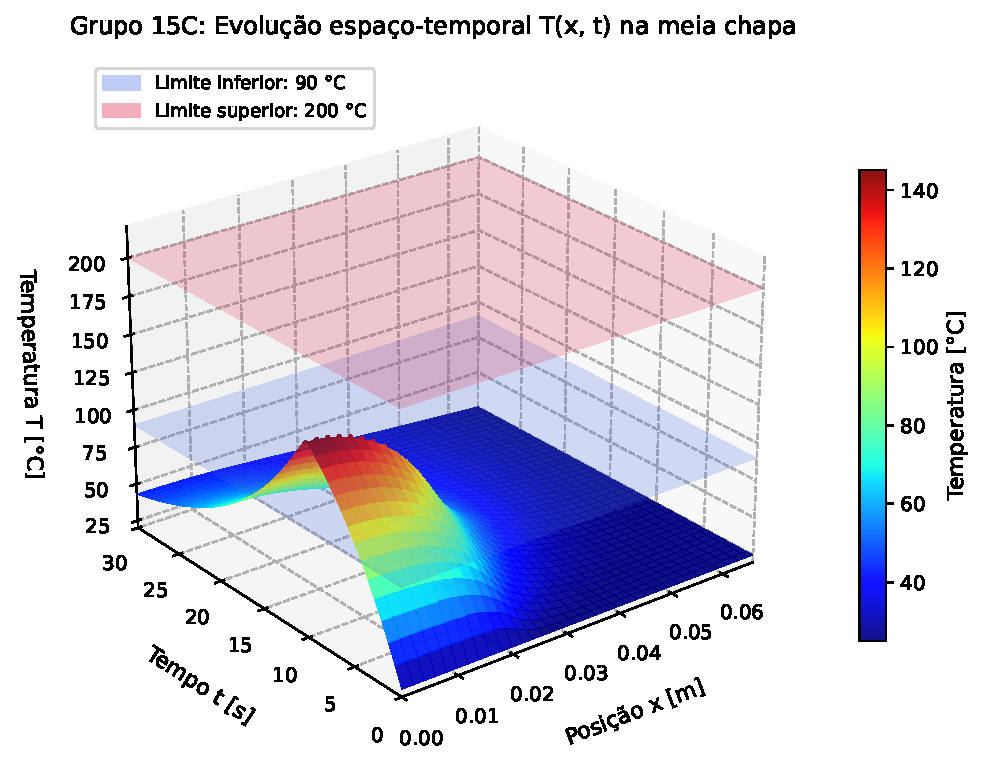
\includegraphics[width=0.84\textwidth]{figuras/fig_superficie_3d.pdf}
    \caption{Superfície tridimensional $T(x,t)$ para o caso base do Grupo 15C na meia chapa ($0 \le x \le \SI{0,066}{m}$, $0 \le t \le \SI{30}{s}$) com planos de referência em \SI{90}{\celsius} e \SI{200}{\celsius}.}
    \label{fig:superficie3d}
\end{figure}

A Figura~\ref{fig:perfis} exibe os perfis espaciais de temperatura em instantes selecionados nas fases de aquecimento ($t \le \SI{10}{s}$) e resfriamento ($t > \SI{10}{s}$), evidenciando o forte gradiente térmico entre o centro e a borda da película ($x = \SI{22}{mm}$) causado pela condução lateral para a zona não irradiada da chapa. A Figura~\ref{fig:temporal} complementa essa análise mostrando o histórico temporal em quatro posições estratégicas ($x = 0$, $11$, $22$ e $\SI{44}{mm}$).

\begin{figure}[H]
    \centering
    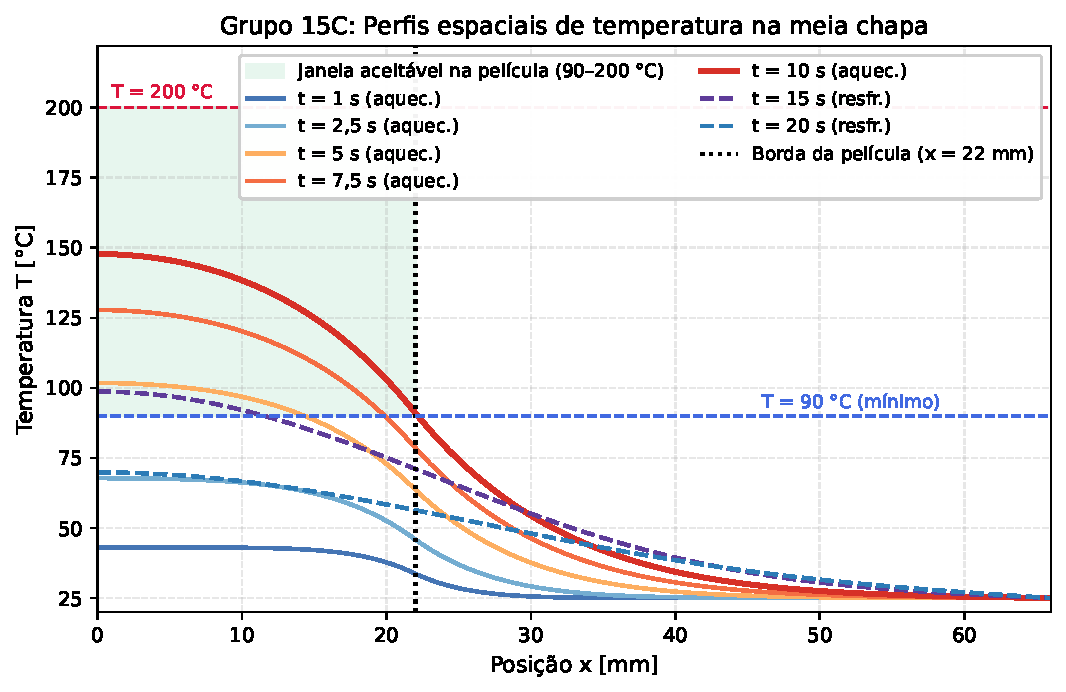
\includegraphics[width=0.86\textwidth]{figuras/fig_perfis_espaciais.pdf}
    \caption{Perfis espaciais $T(x)$ em instantes selecionados de aquecimento e resfriamento para o Grupo 15C.}
    \label{fig:perfis}
\end{figure}

\begin{figure}[H]
    \centering
    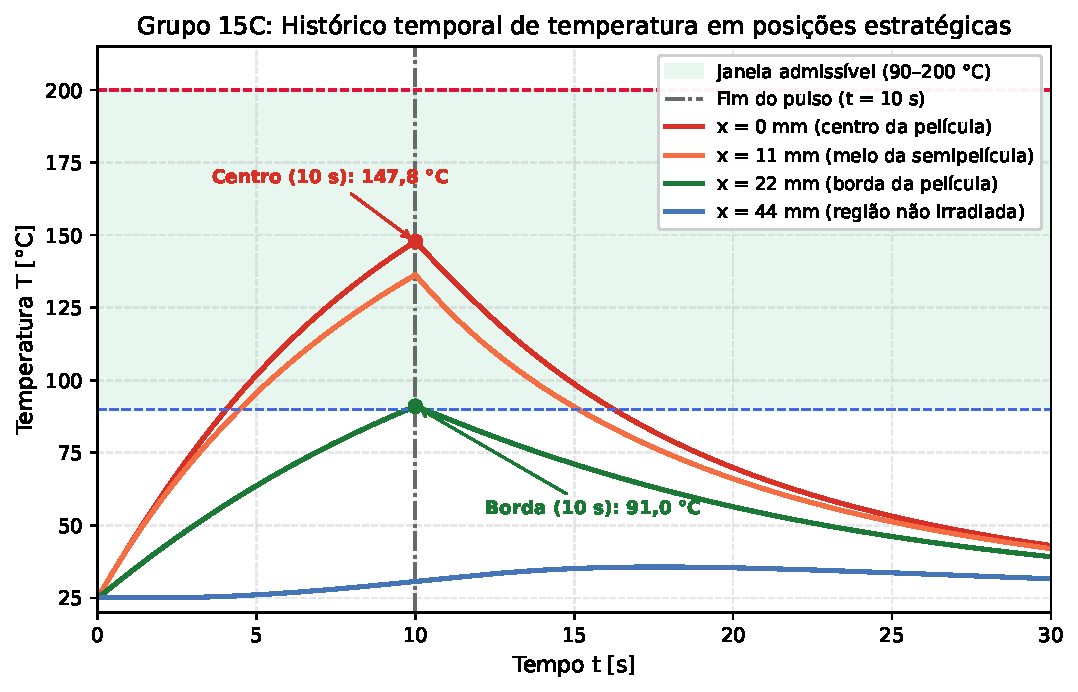
\includegraphics[width=0.86\textwidth]{figuras/fig_evolucao_temporal.pdf}
    \caption{Evolução temporal $T(t)$ em posições estratégicas da chapa para o Grupo 15C, destacando a janela de colagem [\SI{90}{\celsius}, \SI{200}{\celsius}] e o término do pulso em $t = \SI{10}{s}$.}
    \label{fig:temporal}
\end{figure}

Os indicadores quantitativos extraídos da simulação do caso base estão consolidados na Tabela~\ref{tab:resumo_base}.

\begin{table}[H]
    \centering
    \caption{Indicadores térmicos do caso base do Grupo 15C ($N = 200, N_t = 3000$).}
    \label{tab:resumo_base}
    \begin{tabular}{lc}
        \toprule
        \textbf{Grandeza avaliada} & \textbf{Valor obtido} \\
        \midrule
        Temperatura máxima na película ($T_{\max} = T(0, \SI{10}{s})$) & \SI{147,80}{\celsius} \\
        Temperatura em $x = \SI{11}{mm}$ ao fim do pulso ($t = \SI{10}{s}$) & \SI{136,29}{\celsius} \\
        Temperatura mínima na película ($T_{\text{borda}} = T(\SI{22}{mm}, \SI{10}{s})$) & \SI{91,02}{\celsius} \\
        Temperatura fora da película ($T(\SI{44}{mm}, \SI{10}{s})$) & \SI{30,64}{\celsius} \\
        Diferença térmica centro--borda na película ($\Delta T_{\text{pel}}$) & \SI{56,78}{\celsius} \\
        Instante em que o centro atinge \SI{90}{\celsius} ($t_{90,\text{centro}}$) & \SI{4,06}{s} \\
        Instante em que a película inteira ultrapassa \SI{90}{\celsius} ($t_{90,\text{borda}}$) & \SI{9,78}{s} \\
        Tempo útil com toda a película em $[\SI{90}{\celsius}, \SI{200}{\celsius}]$ durante o pulso & \SI{0,224}{s} (\SI{2,2}{\percent} do pulso) \\
        Violação do limite superior ($T > \SI{200}{\celsius}$) & Não (folga de \SI{52,20}{\celsius}) \\
        Resfriamento: centro / borda em $t = \SI{15}{s}$ & \SI{98,70}{\celsius} / \SI{71,09}{\celsius} \\
        Resfriamento: centro / borda em $t = \SI{20}{s}$ & \SI{69,86}{\celsius} / \SI{56,38}{\celsius} \\
        Resfriamento: centro / borda em $t = \SI{30}{s}$ & \SI{43,02}{\celsius} / \SI{39,18}{\celsius} \\
        \bottomrule
    \end{tabular}
\end{table}

\textbf{Diagnóstico crítico do processo atual:} embora a condição de pico máximo não viole o teto de \SI{200}{\celsius} ($T_{\max} = \SI{147,80}{\celsius}$) e a borda da película chegue a cruzar marginalmente o patamar inferior no final do pulso ($T_{\text{borda}}(\SI{10}{s}) = \SI{91,02}{\celsius}$), o processo \textbf{não é tecnicamente satisfatório} em escala industrial pelos seguintes motivos:
\begin{enumerate}
    \item \textbf{Tempo útil irrisório:} enquanto o centro atinge \SI{90}{\celsius} em $t = \SI{4,06}{s}$, a borda ($x = \SI{22}{mm}$) só ultrapassa \SI{90}{\celsius} em $t = \SI{9,78}{s}$, restando apenas \SI{0,224}{s} (\SI{2,24}{\percent} do ciclo de aquecimento) com toda a largura da película simultaneamente dentro da janela de colagem.
    \item \textbf{Margem operacional nula:} a borda excede o limite mínimo em apenas \SI{1,02}{\celsius}. Qualquer pequena flutuação real na potência do laser (\SI{+-2}{\percent}), no coeficiente convectivo local ou na posição do feixe fará a extremidade da película operar abaixo de \SI{90}{\celsius}, causando descolamento nas bordas.
    \item \textbf{Elevada não uniformidade térmica:} o gradiente lateral de \SI{56,78}{\celsius} entre centro e borda decorre do dreno de calor por condução na chapa de aço adjacente ($x > \SI{22}{mm}$), que permanece fria e atua como uma aleta resfriada por convecção elevada ($h = \SI{150}{W/(m^2.K)}$).
\end{enumerate}

% =========================================================================
% 6. PROPOSTA DE SOLUCOES PARA ADEQUACAO DO PROCESSO
% =========================================================================
\section{Proposta de soluções para adequação do processo}

Diante das limitações identificadas no caso base, avaliaram-se numericamente quatro alternativas práticas de engenharia que podem ser implementadas pelo fabricante do sistema laser ou na linha de produção:

\begin{itemize}
    \item \textbf{Solução A -- Ajuste da potência (fluxo $q''$, mantendo $w_{\text{laser}} = \SI{44}{mm}$):} aproveitando a linearidade da equação~\eqref{eq:edp_dim} em $(T - T_\infty)$, calculou-se a faixa teórica de operação entre o mínimo para a borda atingir \SI{90}{\celsius} ($q''_{\min} = \SI{78,76}{kW/m^2}$) e o máximo para o centro não exceder \SI{200}{\celsius} ($q''_{\max} = \SI{114,00}{kW/m^2}$). Adotando o ponto de operação $q'' = \SI{105}{kW/m^2}$ (folga de segurança de \SI{13,82}{\celsius} abaixo de \SI{200}{\celsius}), a borda atinge \SI{90}{\celsius} em $t = \SI{6,77}{s}$, ampliando a janela útil para \SI{3,23}{s}. Contudo, o desnível térmico centro--borda agrava-se para \SI{74,52}{\celsius}.
    \item \textbf{Solução B -- Alargamento do feixe de laser ($w_{\text{laser}} = \SI{60}{mm} > w_1$, com $q'' = \SI{80}{kW/m^2}$):} irradiando uma faixa ligeiramente mais larga que a película ($\SI{8}{mm}$ adicionais em cada lado), o aquecimento suplementar nas regiões adjacentes compensa as perdas por condução lateral na borda da película ($x = \SI{22}{mm}$). Sem elevar o fluxo específico do laser, a borda sobe para \SI{129,70}{\celsius}, o gradiente térmico na película despenca de \SI{56,78}{\celsius} para \SI{26,06}{\celsius}, a folga em relação a \SI{200}{\celsius} permanece ampla (\SI{44,24}{\celsius}) e o tempo útil salta para \SI{5,12}{s} ($t_{90,\text{borda}} = \SI{4,88}{s}$).
    \item \textbf{Solução C -- Pulso em dois estágios associado ao feixe alargado ($w_{\text{laser}} = \SI{60}{mm}$, recomendada):} consiste em programar o controlador do laser com uma rampa inicial de alta potência ($q''_1 = \SI{180}{kW/m^2}$ entre $0 < t \le \SI{2,0}{s}$) seguida de um patamar de manutenção ($q''_2 = \SI{75}{kW/m^2}$ entre $\SI{2,0}{s} < t \le \SI{10,0}{s}$). O primeiro estágio vence rapidamente a inércia térmica da chapa, levando a película inteira acima de \SI{90}{\celsius} em apenas \SI{1,76}{s}, enquanto o segundo estágio estabiliza a colagem entre \SI{140,76}{\celsius} (borda) e \SI{171,37}{\celsius} (centro), garantindo \SI{8,24}{s} úteis dentro do pulso de \SI{10}{s} (\SI{82,4}{\percent} do ciclo) e margem térmica de \SI{28,63}{\celsius} abaixo de \SI{200}{\celsius}.
    \item \textbf{Solução D -- Pré-aquecimento da chapa ($T_0 = \SI{55}{\celsius}$) ou redução de convecção:} o pré-aquecimento inicial para \SI{55}{\celsius} (com $q'' = \SI{80}{kW/m^2}$ e $w_{\text{laser}} = \SI{44}{mm}$) eleva a borda para \SI{105,60}{\celsius} e gera \SI{3,91}{s} de janela útil, mas mantém elevado gradiente (\SI{57,05}{\celsius}) e exige forno/aquecedor auxiliar na linha do cliente. Ressalta-se que, nessa simulação, a condição de contorno na extremidade da fita ($x = \SI{66}{mm}$) foi mantida em $T_\infty = \SI{25}{\celsius}$, sem impacto prático sobre a região da película ($|x| \le \SI{22}{mm}$) no intervalo de \SI{10}{s}. De forma análoga, uma carenagem que reduzisse a convecção de $h = \SI{150}{W/(m^2.K)}$ para $h = \SI{100}{W/(m^2.K)}$ elevaria a borda apenas para \SI{98,41}{\celsius} e o tempo útil para \SI{1,42}{s}, mostrando-se insuficiente isoladamente.
\end{itemize}

A Tabela~\ref{tab:solucoes} compara quantitativamente todas as configurações simuladas, e a Figura~\ref{fig:comparacao} ilustra o ganho expressivo de uniformidade espacial e de tempo útil de colagem obtido pelas soluções propostas.

\begin{table}[H]
    \centering
    \caption{Comparação quantitativa entre o caso base e as soluções de engenharia simuladas para o Grupo 15C.}
    \label{tab:solucoes}
    \footnotesize
    \setlength{\tabcolsep}{4pt}
    \begin{tabular}{lcccccc}
        \toprule
        \textbf{Cenário} &
        \cab{$T_{\max}$}{{[$^\circ\text{C}$]}} &
        \cab{$T_{\text{borda}}(\SI{10}{s})$}{{[$^\circ\text{C}$]}} &
        \cab{$\Delta T_{\text{pel}}$}{{[$^\circ\text{C}$]}} &
        \cab{$t_{90,\text{borda}}$}{{[s]}} &
        \cab{\textbf{Janela útil}}{{[s]}} &
        \cab{\textbf{Margem \SI{200}{\celsius}}}{{[$^\circ\text{C}$]}} \\
        \midrule
        Caso base ($80\text{ kW/m}^2$, $44\text{ mm}$) & \num{147,80} & \num{91,02} & \num{56,78} & \num{9,78} & \num{0,22} & \num{52,20} \\
        Sol. A ($105\text{ kW/m}^2$, $44\text{ mm}$) & \num{186,18} & \num{111,65} & \num{74,52} & \num{6,77} & \num{3,23} & \num{13,82} \\
        Sol. B ($w_L=\SI{60}{mm}$, $80\text{ kW/m}^2$) & \num{155,76} & \num{129,70} & \num{26,06} & \num{4,88} & \num{5,12} & \num{44,24} \\
        \textbf{Sol. C (2 estágios + $\SI{60}{mm}$)} & \textbf{\num{171,37}} & \textbf{\num{140,76}} & \textbf{\num{30,61}} & \textbf{\num{1,76}} & \textbf{\num{8,24}} & \textbf{\num{28,63}} \\
        Sol. D (pré-aquec. $T_0=\SI{55}{\celsius}$) & \num{162,65} & \num{105,60} & \num{57,05} & \num{6,09} & \num{3,91} & \num{37,35} \\
        Carenagem ($h=\SI{100}{W/(m^2.K)}$) & \num{160,71} & \num{98,41} & \num{62,30} & \num{8,58} & \num{1,42} & \num{39,29} \\
        \bottomrule
    \end{tabular}
\end{table}

\begin{figure}[H]
    \centering
    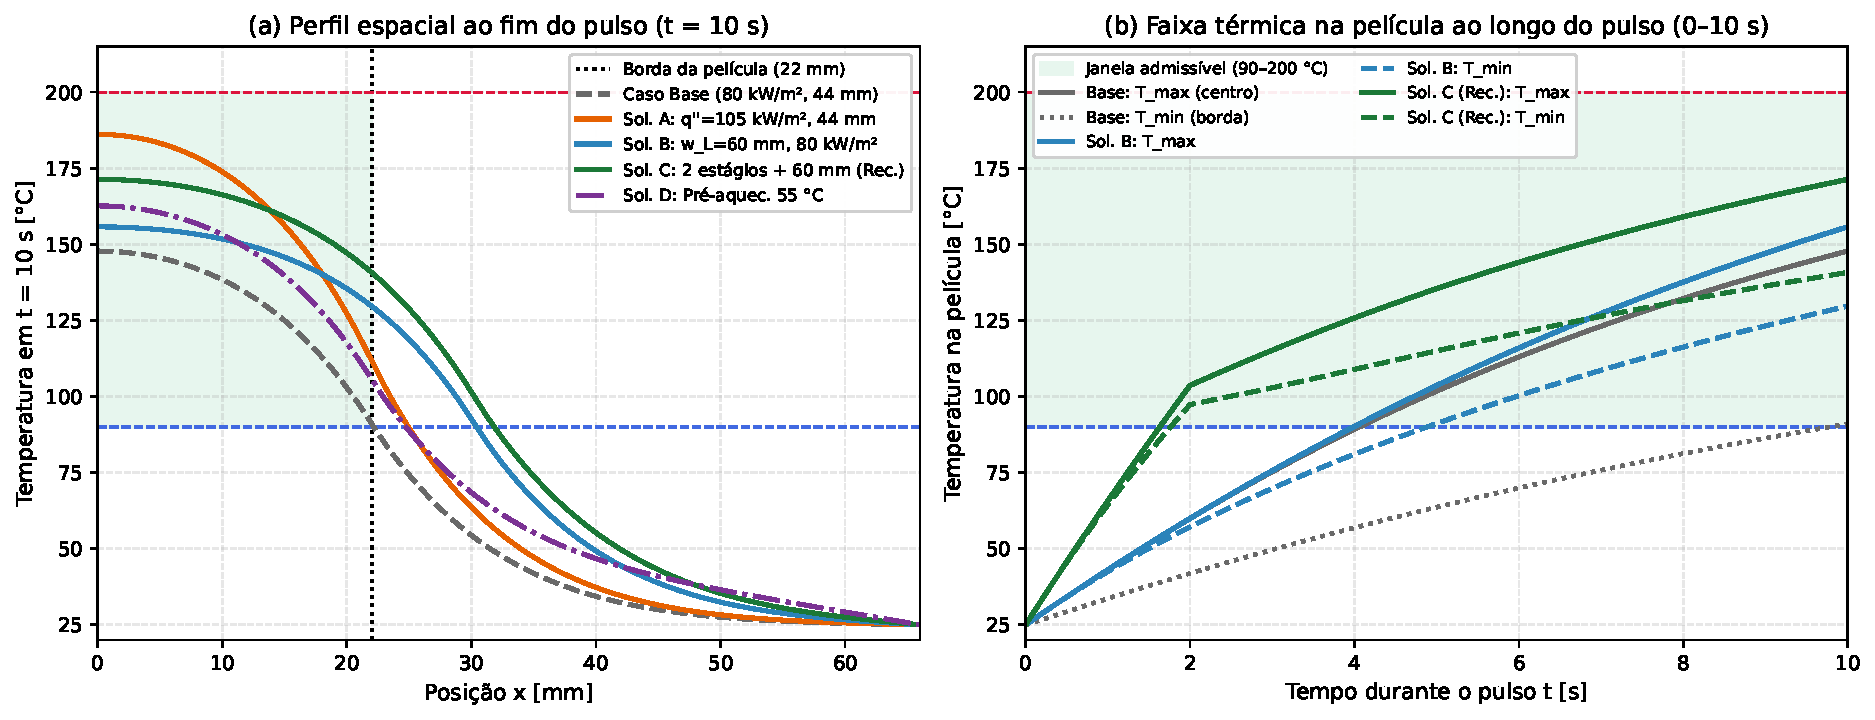
\includegraphics[width=\textwidth]{figuras/fig_comparacao_solucoes.pdf}
    \caption{Comparação entre o caso base do Grupo 15C e as soluções propostas: (a) perfis espaciais ao término do pulso ($t = \SI{10}{s}$) e (b) envoltório térmico ($T_{\max}$ e $T_{\min}$) sobre a película durante o intervalo de $\SI{10}{s}$.}
    \label{fig:comparacao}
\end{figure}

\textbf{Recomendação técnica:} recomenda-se à empresa fornecedora do sistema a adoção da \textbf{Solução C (pulso em dois estágios com feixe alargado para $w_{\text{laser}} = \SI{60}{mm}$)}, por multiplicar por \textbf{36,7 vezes} o tempo útil de colagem (\SI{8,24}{s} contra \SI{0,224}{s} no caso base), manter toda a película em faixa homogênea ($140{,}8$ a $\SI{171,4}{\celsius}$) com folga robusta tanto acima de \SI{90}{\celsius} quanto abaixo de \SI{200}{\celsius}, e requerer apenas ajuste óptico do colimador e modulação temporal do laser sem alterações no ambiente convectivo da linha. Caso a fonte laser não disponha de modulação temporal em dois patamares, a \textbf{Solução B ($w_{\text{laser}} = \SI{60}{mm}$ com $q''$ constante)} constitui a melhor alternativa passiva (\SI{5,12}{s} de janela útil e menor gradiente espacial, $\Delta T_{\text{pel}} = \SI{26,06}{\celsius}$).

% =========================================================================
% 7. CONCLUSOES
% =========================================================================
\section{Conclusões}
O estudo numérico do processo de colagem por laser para o \textbf{Grupo 15C} permitiu concluir que:
\begin{enumerate}
    \item A modelagem unidimensional transiente é plenamente justificada pelo baixo número de Biot transversal ($\text{Bi}_y = \num{3,125e-3} \ll 0,1$), e o esquema implícito em diferenças finitas com condição de simetria de Lomax e Pulliam mostrou-se preciso e estável, reproduzindo fielmente o \textit{benchmark} do Grupo 11A e apresentando convergência espacial e temporal inferior a \SI{1}{\percent} na malha base ($N=200, N_t=3000$).
    \item Na configuração original do Grupo 15C ($h = \SI{150}{W/(m^2.K)}$, $q'' = \SI{80}{kW/m^2}$, $T_\infty = \SI{25}{\celsius}$), embora o centro alcance \SI{147,80}{\celsius} sem superar \SI{200}{\celsius}, a condução lateral limita a borda da película a \SI{91,02}{\celsius} ao final do pulso, gerando uma janela útil de apenas \SI{0,224}{s} e tornando o processo inadequado para operação industrial confiável.
    \item A simples elevação da potência com feixe de $\SI{44}{mm}$ (Solução A) possui margem estreita antes de violar \SI{200}{\celsius} ($q''_{\max} = \SI{114,0}{kW/m^2}$) e acentua o gradiente térmico ($\Delta T_{\text{pel}} = \SI{74,52}{\celsius}$).
    \item O alargamento do feixe para $w_{\text{laser}} = \SI{60}{mm}$ combinado ao pulso em dois estágios ($\SI{180}{kW/m^2}$ por $\SI{2,0}{s}$ + $\SI{75}{kW/m^2}$ até $\SI{10,0}{s}$, Solução C) resolve integralmente o problema: reduz o gradiente na película para \SI{30,61}{\celsius}, mantém \SI{28,63}{\celsius} de margem de segurança abaixo de \SI{200}{\celsius} e assegura \SI{8,24}{s} de permanência plena na janela de colagem.
\end{enumerate}

% =========================================================================
% REFERENCIAS
% =========================================================================
\begin{thebibliography}{9}
    \bibitem{volpe} VOLPE, E.~V. \textit{Notas de Aula de PME 3361 -- Transferência de Calor: Formulação e Método Numérico do Projeto I}. Escola Politécnica da Universidade de São Paulo, 2026.
    \bibitem{incropera} BERGMAN, T.~L.; LAVINE, A.~S.; INCROPERA, F.~P.; DEWITT, D.~P. \textit{Fundamentos de Transferência de Calor e de Massa}. 8. ed. Rio de Janeiro: LTC, 2019.
    \bibitem{lomax} LOMAX, H.; PULLIAM, T.~H.; ZINGG, D.~W. \textit{Fundamentals of Computational Fluid Dynamics}. Berlin: Springer, 2001.
\end{thebibliography}

% =========================================================================
% APENDICE A - CODIGO-FONTE
% =========================================================================
\newpage
\appendix
\section{Código-fonte da simulação}
\label{ap:codigo}
Abaixo encontra-se o código integral em Python (\texttt{simulacao.py}) empregado na validação do \textit{benchmark}, no estudo de convergência de malha, nas simulações do caso base e na avaliação das soluções de engenharia do Grupo 15C.

\lstinputlisting[language=Python, caption={Script principal de simulação numérica e geração de gráficos (\texttt{simulacao.py}).}]{simulacao.py}

\end{document}
